Em 2014 foi inaugurada a maior roda-gigante do mundo, a High Roller, situada em Las Vegas. A figura representa um esbo�o dessa roda-gigante, no qual o ponto A representa uma de suas cadeiras: 

\begin{figure}[h]
\centering
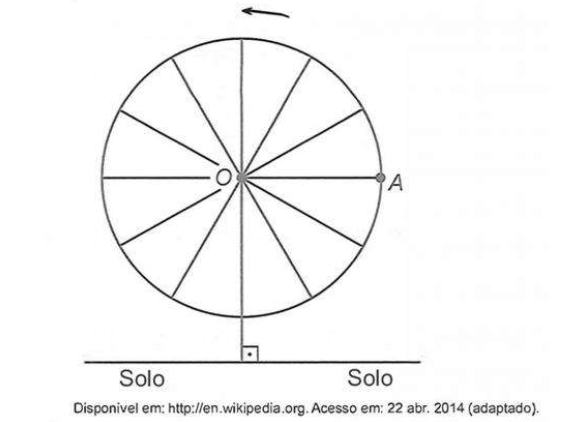
\includegraphics[width=8cm]{../figuras/q154(1)-2018.png}
\end{figure}

A partir da posi��o indicada, em que o segmento OA se encontra paralelo ao plano do solo, rotaciona-se a High Roller no sentido anti-hor�rio, em torno do ponto O. Sejam t o �ngulo determinado pelo segmento OA em rela��o � sua posi��o inicial, e f a fun��o que descreve a altura do ponto A, em rela��o ao solo, em fun��o de t. Ap�s duas voltas completas, f tem o seguinte gr�fico:
\begin{figure}[h]
\centering
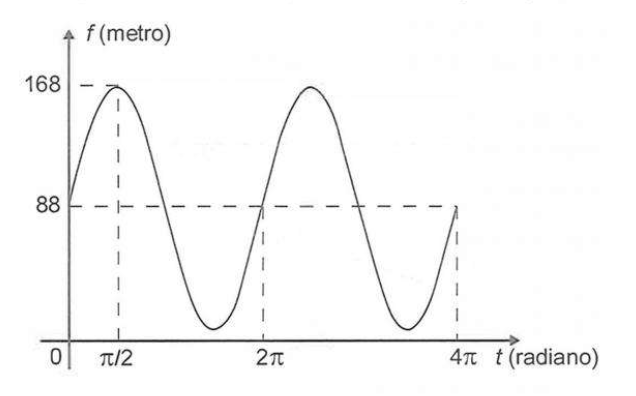
\includegraphics[width=8cm]{../figuras/q154(2)-2018.png}
\end{figure}
A express�o da fun��o altura � dada por 
\begin{enumerate}
\item[a)]$f(t)=80sen(t)+88$
\item[b)]$f(t)=80cos(t)+88$
\item[c)]$f(t)=88cos(t)+88$
\item[d)]$f(t)=168sen(t)+88cos(t)$
\item[e)]$f(t)=88sen(t)+168cos(t)$
\end{enumerate}